%% LyX 2.3.2 created this file.  For more info, see http://www.lyx.org/.
%% Do not edit unless you really know what you are doing.
\documentclass[english]{article}
\usepackage[T1]{fontenc}
\usepackage[latin9]{inputenc}
\usepackage{color}
\usepackage{verbatim}
\usepackage{float}
\usepackage{amsmath}
\usepackage{amsthm}
\usepackage{mathptmx}
\usepackage{newtxmath}
\usepackage{graphicx}
\PassOptionsToPackage{normalem}{ulem}
\usepackage{ulem}

\makeatletter
%%%%%%%%%%%%%%%%%%%%%%%%%%%%%% User specified LaTeX commands.
\usepackage{mathptmx}
\usepackage{newtxmath}
\renewcommand{\familydefault}{\rmdefault}
\usepackage[T1]{fontenc}
\usepackage{geometry}
\geometry{verbose,tmargin=2.5cm,bmargin=2.5cm,lmargin=2.5cm,rmargin=2.5cm}
\usepackage{color}
\usepackage{array}
\usepackage{verbatim}
\usepackage{float}
\usepackage{rotfloat}
\usepackage{booktabs}
\usepackage{bm}
\usepackage{graphicx}
\usepackage{setspace}
\doublespacing

\makeatletter

%%%%%%%%%%%%%%%%%%%%%%%%%%%%%% LyX specific LaTeX commands.
%% Because html converters don't know tabularnewline
\providecommand{\tabularnewline}{\\}

%%%%%%%%%%%%%%%%%%%%%%%%%%%%%% Textclass specific LaTeX commands.
\theoremstyle{plain}
\newtheorem{thm}{\protect\theoremname}[section]
\theoremstyle{plain}
\newtheorem{prop}[thm]{\protect\propositionname}

\@ifundefined{date}{}{\date{}}
%%%%%%%%%%%%%%%%%%%%%%%%%%%%%% User specified LaTeX commands.




\usepackage{amsthm}
\theoremstyle{definition}
\newtheorem{definition}{Definition}[section]

\usepackage{cleveref}
\usepackage{algorithmic}
\usepackage{array}
\usepackage{stfloats}
\usepackage[super]{nth}
\usepackage{subcaption}
\usepackage{caption}
% for inkscape images
\usepackage{xcolor}
\usepackage{tikz}
\usepackage{pgf}


\g@addto@macro\@floatboxreset\centering


% \usepackage{hyperref}
 
 \AtBeginDocument{% Overrides ref for Cref
 	\let\ref\Cref
 }

\crefalias{prop}{proposition}

% TIKZ
\usepackage{tikz}

% -- Arrows
\usetikzlibrary{arrows}

% --Bayesnet
\usetikzlibrary{bayesnet}
\usetikzlibrary{decorations.pathreplacing}

\tikzset{
	diagonal fill/.style 2 args={fill=#2, path picture={
			\fill[#1, sharp corners] (path picture bounding box.south west) -|
			(path picture bounding box.north east) -- cycle;}},
	reversed diagonal fill/.style 2 args={fill=#2, path picture={
			\fill[#1, sharp corners] (path picture bounding box.north west) |- 
			(path picture bounding box.south east) -- cycle;}}
}

\tikzstyle{partialobs} = [latent,diagonal fill={gray!25}{gray!0}]

%\@ifundefined{showcaptionsetup}{}{%
% \PassOptionsToPackage{caption=false}{subfig}}
%\usepackage{subfig}
%\makeatother

\providecommand{\propositionname}{Proposition}
\providecommand{\theoremname}{Theorem}

\usepackage[style=chicago-authordate,isbn=false,url=false,eprint=false,minbibnames=10, maxbibnames=10,maxcitenames=3,firstinits=true]{biblatex}
\DeclareFieldFormat[article,inbook,book,incollection,inproceedings,patent,thesis,unpublished]{citetitle}{#1}
\DeclareFieldFormat[article,inbook,incollection,inproceedings,patent,thesis,unpublished]{title}{#1} 

\providecommand{\propositionname}{Proposition}
\providecommand{\theoremname}{Theorem}

\addbibresource{bibliography.bib}

% # PAPER SPECIFIC
\global\long\def\Tsq{T^{2}}%
\global\long\def\priordist{p_{z}}%
\global\long\def\detencoding{g_{\mbphi}}%
\global\long\def\detdecoding{f_{\mbtheta}}%
\global\long\def\encoding{q_{\mbphi}(\mbz\g\mbx)}%
\global\long\def\decoding{p_{\mbtheta}(\mbx\g\mbz)}%
\global\long\def\czero{c_{0}}%
\global\long\def\dataset{\mathcal{D}}%
\global\long\def\mbxover#1{\mbx^{(#1)}}%
\global\long\def\stdGauss{\Norm(\mbzero, \mbI)}%
\global\long\def\pdata{p_{data}(x)}%
\global\long\def\ptheta{p_{\mbtheta}}%
\global\long\def\pthetaxgivenz#1#2{\ptheta(#1 \g#2)}%
\global\long\def\qphi{q_{\mbphi}}%
\global\long\def\qphizgivenx#1#2{\qphi(#1 \g#2)}%
\global\long\def\pz{p(\mbz)}%
\global\long\def\oursacronym{SPE}%
\global\long\def\TsqKLD{T_{\mathrm{KLD}}^{2}}%
\global\long\def\QERE{Q_{\mathrm{ERE}}}%
% # TYPOGRAPHY
\global\long\def\etal{\textit{et al}. }%
\global\long\def\ie{\textit{i}.\textit{e}.}%
\global\long\def\eg{\textit{e}.\textit{g}.}%
% # PROBABILITY

\global\long\def\g{\,|\,}%
\global\long\def\gg{\,\|\,}%
\global\long\def\KL#1#2{\textrm{KL}\left(#1\gg#2\right)}%
\global\long\def\E{\mathbb{E}}%
% Expectation

% # DISTRIBUTIONS

\global\long\def\Norm{\mathcal{N}}%
% Gaussian likelihood
\global\long\def\Gam{\textrm{Gam}}%
\global\long\def\InvGam{\textrm{InvGam}}%
% # MISCELLANEOUS

\global\long\def\d#1{\ensuremath{\operatorname{d}\!{#1}}}%
\global\long\def\diag{\textrm{diag}}%
\global\long\def\supp{\textrm{supp}}%
\global\long\def\indep{\mathpalette{\independenT}{\perp}}%
\global\long\def\independenT#1#2{\mathrel{\rlap{$#1#2$}\mkern2mu  {#1#2}}}%
\global\long\def\inv{^{\raisebox{.2ex}{${\scriptscriptstyle -1}$}}}%

% # SET NOTATION
\global\long\def\R{\mathbb{R}}%
% # BOLD MATHEMATICS

\global\long\def\mba{\bm{a}}%
\global\long\def\mbb{\bm{b}}%
\global\long\def\mbc{\bm{c}}%
\global\long\def\mbd{\bm{d}}%
\global\long\def\mbe{\bm{e}}%
%\newcommand{\mbf}{\bm{f}}
\global\long\def\mbg{\bm{g}}%
\global\long\def\mbh{\bm{h}}%
\global\long\def\mbi{\bm{i}}%
\global\long\def\mbj{\bm{j}}%
\global\long\def\mbk{\bm{k}}%
\global\long\def\mbl{\bm{l}}%
\global\long\def\mbm{\bm{m}}%
\global\long\def\mbn{\bm{n}}%
\global\long\def\mbo{\bm{o}}%
\global\long\def\mbp{\bm{p}}%
\global\long\def\mbq{\bm{q}}%
\global\long\def\mbr{\bm{r}}%
\global\long\def\mbs{\bm{s}}%
\global\long\def\mbt{\bm{t}}%
\global\long\def\mbu{\bm{u}}%
\global\long\def\mbv{\bm{v}}%
\global\long\def\mbw{\bm{w}}%
\global\long\def\mbx{\bm{x}}%
\global\long\def\mby{\bm{y}}%
\global\long\def\mbz{\bm{z}}%
\global\long\def\mbA{\bm{A}}%
\global\long\def\mbB{\bm{B}}%
\global\long\def\mbC{\bm{C}}%
\global\long\def\mbD{\bm{D}}%
\global\long\def\mbE{\bm{E}}%
\global\long\def\mbF{\bm{F}}%
\global\long\def\mbG{\bm{G}}%
\global\long\def\mbH{\bm{H}}%
\global\long\def\mbI{\bm{I}}%
\global\long\def\mbJ{\bm{J}}%
\global\long\def\mbK{\bm{K}}%
\global\long\def\mbL{\bm{L}}%
\global\long\def\mbM{\bm{M}}%
\global\long\def\mbN{\bm{N}}%
\global\long\def\mbO{\bm{O}}%
\global\long\def\mbP{\bm{P}}%
\global\long\def\mbQ{\bm{Q}}%
\global\long\def\mbR{\bm{R}}%
\global\long\def\mbS{\bm{S}}%
\global\long\def\mbT{\bm{T}}%
\global\long\def\mbU{\bm{U}}%
\global\long\def\mbV{\bm{V}}%
\global\long\def\mbW{\bm{W}}%
\global\long\def\mbX{\bm{X}}%
\global\long\def\mbY{\bm{Y}}%
\global\long\def\mbZ{\bm{Z}}%
\global\long\def\mbalpha{\bm{\alpha}}%
\global\long\def\mbbeta{\bm{\beta}}%
\global\long\def\mbdelta{\bm{\delta}}%
\global\long\def\mbepsilon{\bm{\epsilon}}%
\global\long\def\mbchi{\bm{\chi}}%
\global\long\def\mbeta{\bm{\eta}}%
\global\long\def\mbgamma{\bm{\gamma}}%
\global\long\def\mbiota{\bm{\iota}}%
\global\long\def\mbkappa{\bm{\kappa}}%
\global\long\def\mblambda{\bm{\lambda}}%
\global\long\def\mbmu{\bm{\mu}}%
\global\long\def\mbnu{\bm{\nu}}%
\global\long\def\mbomega{\bm{\omega}}%
\global\long\def\mbphi{\bm{\phi}}%
\global\long\def\mbpi{\bm{\pi}}%
\global\long\def\mbpsi{\bm{\psi}}%
\global\long\def\mbrho{\bm{\rho}}%
\global\long\def\mbsigma{\bm{\sigma}}%
\global\long\def\mbtau{\bm{\tau}}%
\global\long\def\mbtheta{\bm{\theta}}%
\global\long\def\mbupsilon{\bm{\upsilon}}%
\global\long\def\mbvarepsilon{\bm{\varepsilon}}%
\global\long\def\mbvarphi{\bm{\varphi}}%
\global\long\def\mbvartheta{\bm{\vartheta}}%
\global\long\def\mbvarrho{\bm{\varrho}}%
\global\long\def\mbxi{\bm{\xi}}%
\global\long\def\mbzeta{\bm{\zeta}}%
\global\long\def\mbDelta{\bm{\Delta}}%
\global\long\def\mbGamma{\bm{\Gamma}}%
\global\long\def\mbLambda{\bm{\Lambda}}%
\global\long\def\mbOmega{\bm{\Omega}}%
\global\long\def\mbPhi{\bm{\Phi}}%
\global\long\def\mbPi{\bm{\Pi}}%
\global\long\def\mbPsi{\bm{\Psi}}%
\global\long\def\mbSigma{\bm{\Sigma}}%
\global\long\def\mbTheta{\bm{\Theta}}%
\global\long\def\mbUpsilon{\bm{\Upsilon}}%
\global\long\def\mbXi{\bm{\Xi}}%
\global\long\def\mbzero{\bm{0}}%
\global\long\def\mbone{\bm{1}}%
\global\long\def\mbtwo{\bm{2}}%
\global\long\def\mbthree{\bm{3}}%
\global\long\def\mbfour{\bm{4}}%
\global\long\def\mbfive{\bm{5}}%
\global\long\def\mbsix{\bm{6}}%
\global\long\def\mbseven{\bm{7}}%
\global\long\def\mbeight{\bm{8}}%
\global\long\def\mbnine{\bm{9}}%



\makeatother

\usepackage{babel}
\begin{document}
\title{Response to ``Toward a Better Monitoring Statistic for Profile Monitoring
with Variational Autoencoders''}
\maketitle

\section{Overall Comments}

Your article has been reviewed by two reviewers and I, as guest-editor
of the JQT Special Issue. Reports from the two reviewers are below.
The decision for this article is Major Revision. Specifically, Reviewer
1 viewed the paper positively, but expressed concerns about the generalizability
of your method. This reviewer asks you to consider other architectures
besides convolutional neural networks to evaluate the generality of
your method. Reviewer 2 was less positive. This reviewer expressed
concerns about the ability for the JQT audience to understand your
paper, and also points out several important technical issues that
should be addressed. The guest editor did not provide a report, but
agreed that the paper addresses an important topic, and is a good
fit with the direction of the JQT Special Issue on Artificial Intelligence.
The guest editor concurs with the technical and editorial suggestions
of both reviewers. I encourage you to submit a revision of this article,
and when doing so, please include a point-by-point response to each
of the reviewers\textquoteright{} concerns.

\textbf{\uline{Ans: }}Thank you for the great suggestions. According
to the reviewers' comments, we have made the following revision to
the paper
\begin{itemize}
\item Revision 1
\item Revision 2.
\item List the overview of your revisions after finishing the paper.
\end{itemize}

\section{Reviewer: 1}

\subsection{Major Comments}

This paper is well written and the technical details describing variational
autoencoders, classical SPC monitoring, deep learning architectures
and proposed statistics are well founded and nicely laid out. It is
my belief that the paper, as currently written, deserves acceptance
and publication in this journal. There are a few minor concerns that
might enhance the applicability of the proposed methodology and are
laid out below:
\begin{enumerate}
\item Neural Network Architectures and Training: The authors propose convolutional
neural networks. (CNNs) for both the encoders and decoders. The specific
proposed architectures include Leaky ReLU activation functions with
a negative slope of 0.2. The authors also use stochastic gradient
decent with a batch size of 64 trained for 1000 epochs and a learning
rate of 0.001. My main concern here is that this specific architecture
might work well for certain problems but may not generalize well in
all situations. I consider the authors should explain whether the
proposed methodology is either robust to these hyperparameters, or
if hyperparameter optimization might be required for other problems.

\textbf{\uline{Ans:}} Thank you for this important comment. We
made the following changes to Section3.4:
\begin{itemize}
\item We added the reference on which we base our CNN architecture\cite{higgins2017beta}.
\item We added the reference for why we chose Leaky ReLU with a negative
slope of 0.2 for activation \cite{radford2015unsupervised}.
\item We added the reference on which we base the parameters for Adam optimizer
\cite{KingmaB14}.
\item We added a paragraph in which we explain the rationale behind our
choice of how hyperparameters are fixed. We claim that the selection
is robust since the same setting worked well for two datasets that
are drastically different: the simulation set and the case study.
We state that our choices are based on the VAE convergence and we
provide advise to the practitioners that if they need make adjustments,
they should do it with respect to this indicator.
\end{itemize}
As a result, the following paragraphs are added to Section 3.4:

\textcolor{red}{The sequential order of the computational graphs used
for this study is summarized in . The architecture choice is directly
based on the encoder-decoder architecture that was used in \cite{higgins2017beta},
except that we use Leaky ReLU with a negative slope of 0.2 as the
activation which is advised in \cite{radford2015unsupervised} for
better gradient flow. The encoder outputs nodes, which is a concatenation
of the inferred posterior mean and variance , both are of length .
The number of epochs per training is fixed at and the learning rate
and batch size are fixed at and , respectively, both are chosen empirically
to guarantee a meaningful convergence. Adam algorithm is used for
first-order gradient optimization with parameters as advised in \cite{KingmaB14}.
The model checkpoint is saved at every epoch where a better validation
loss is observed. The latest checkpoint is used as the final model.}

\textcolor{red}{In our experiments, the architecture and the training
conditions described above are generated with respect to the convergence
of the VAE objective on in-control dataset because in real life, the
practitioner will not have access to out-of-control samples. The same
setting worked well for both the simulation dataset and the case study
dataset we consider in this paper. This gives us confidence that the
selection is robust from one set to the other. However, a different
dataset might benefit from adjustments to the above conditions. The
adjustments should be based on monitoring the convergence of the VAE
objective, as the procedure will benefit from a better approximated
in-control distribution.}
\item For sequence-based data other architectures could provide advantages,
such as a Long-Short Term Memory (LSTM) autoencoders. Variational
LSTM autoencoders have been proposed in the literature. I think the
authors should mention whether the proposed statistic could be obtained
using other architectures (besides CNNs) for generality of the methodology.

\textbf{\uline{Ans:}} Thank you for the suggestion. Indeed, we
agree that sequence-based profiles are commonly found and so the possibility
of a recurrent architecture should be mentioned for interested readers.

\begin{itemize}
	\item We added a related note for our readers in the last three paragraphs
	of Section 3.4 as highlighted below in red.
\end{itemize}

\textcolor{red}{Image profiles comprise our simulation and case study,
which will be introduced to the reader in the upcoming sections. This
is why we only consider convolutional architectures. However, the
monitoring statistics we propose in Equation (10) and Equation (11)
are adaptable to other flavors of VAE architectures as well.}

\textcolor{red}{The original VAE \cite{Kingma2013-dl} was introduced
with fully connected feed- forward neural networks which are generally
applicable to most kinds of process inputs. The monitoring statistics
we proposed can be readily applied for that scenario without the need
for further modification.}

\textcolor{red}{For sequential profiles (e.g. time series), two alternative
solutions can be used. First would be using one-dimensional convolutional
layers. In that scenario, since we are still in the realm of convolutional
architectures, no further modifications are needed. Alternatively,
a recurrent neural network-based encoder and decoder structure might
be efficient at capturing sequential dependencies, as outlined in
Chung et al. (2015). A modification required for that method would
be using a variational layer only between the last hidden state of
the encoder and the initial generating state of the decoder, as opposed
to having a VAE at every time step. In other words, the recurrent
layers would be used as a way to encode the sequence-dependent signal
into a vector, just as convolutional layers do the same for spatially-dependent
signal. Given that modification, the proposed monitoring statistics
can be used right away.}
\item The authors mention that the accuracy and computational feasibility
of the proposed method, however for the sake of completeness briefly
explain how computationally demanding is the proposed method and the
computational limitations. With this comment I am not necessarily
referring to the theoretical computational complexity of VAEs, or
of the profile monitoring procedure, but, for example, under a specific
machine configuration and computational power the methodology certain
computational time, and if there are limits in either image size,
sample size, batch size, learning rate, etc.

\textbf{Ans: }Thank you for this suggestion.

\begin{itemize}
	\item We added the a related paragraph at the end of Section 5, which is highlighted below.
\end{itemize} 

\textcolor{red}{Finally, we report execution time on our specific
machine configuration with respect to this case study. For this study,
we utilized a workstation with 6-core Intel(R) Core(TM) i7-5930K CPU
@ 3.50GHz CPUs and 4 GeForce GTX 1080 Ti GPUs. Neural network computations
are executed on a single GPU and a single CPU core is used for image
input/output and preprocessing steps such as resizing to 64-by-64
and grayscale conversion wherever needed. A single GPU has 12GB memory
and the model parameters take up about 730MBs. GPUs can leverage parallel
computation of multiple images, therefore the remaining memory can
be used to stock up images so their execution becomes parallel. An
example of a batch of 128 images take up only 63MBs more space in
the GPU's memory and the per image execution time is roughly 0.8 milliseconds.
On the extreme case of using a single image per batch, average per
image execution time is around 2 milliseconds.}
\item Minor comments
\begin{itemize}
\item Introduction, Page 3, Line 39\dots{} it normally requires many trial
and error CHANGE TO it normally requires trial and error OR rephrase
\item Methodology, Proposition 3.1, Page 12, Line 26 \dots . Where C1 and
C2 and constants that doesn\textquoteright t depend on x CHANGE TO
where C1 and C2 are constants that do not depend on x
\item Comparison of Detection Performance of Proposed Statistics, Page 25,
Line 47 \dots{} the former three is that they don\textquoteright t
rely on random samples CHANGE TO the former three is that they do
not rely on random samples.
\end{itemize}
\textbf{\uline{Ans:}} Thank you for the detailed revision of the
paper. We have made the changes accordingly and carefully proofread
the rest of the paper again.
\end{enumerate}

\section{Reviewer: 2}
\begin{enumerate}
\item I like the intuition that is conveyed regarding why (9) by itself
is not a good monitoring statistic and how (10) overcomes this. My
primary concern is that the paper is not written with the JQT audience
in mind and assumes readers are more familiar with VAE and deep learning
concepts than typical JQT readers are. I hope that the authors can
improve upon this aspect, since I think it could make a nice contribution
to JQT. Many of my comments below relate to this.

\textbf{\uline{Ans:}} We have revised the paper accordingly, with
the consideration of the JQT audience in mind. Please see the detailed
list of revisions below.
\begin{itemize}
\item We have added a new Section 3.1 \textcolor{black}{``Relationship
of the Monitoring Statistics for VAE and PCA'' to link the monitoring
statistics of the PCA and VAE models. with a new figure to illustrate
the analogy between VAE and PCA. The detailed discussion is provided
in the answer to Comment \#3.}
\item We have changed the original figure to explain the concepts of entanglement
with more focus on the incorrect mapping of the latent space as follows
to better explain the concept of the ``incorrect mapping of the latent
space'' phenomena. The detailed \textcolor{black}{discussion} is
provided in the answer to Comment \#4
\item We have removed some of the original discussions about the disentanglement,
which we found also misleading and hard to interpret. The detailed
\textcolor{black}{discussion} is provided in the answer to Comment
\#8.
\item We have revised Figure 2 completely in the paper to demonstrate why
the ``latent space statistics'' would not work. We hope that this
visual illustration would be much easier to understand for the JQT
audiences. The detailed \textcolor{black}{discussion} is provided
in the answer to Comment \#7.
\end{itemize}
\item The writing is very sloppy. Even the very first sentence of the abstract
is incomplete and clearly was not proofread. There are also a lot
of typos and other careless mistakes, e.g., inconsistencies in the
list of references, like some names being replaced by et al. The writing
must be improved to be suitable for JQT.

\textbf{\uline{Ans:}} Thank you for pointing out our writing issues.
We have proofread the papers again and all the revision of the papers
are highlighted in the revised manuscript. The references are updated
according to ``Taylor \& Francis US Chicago (B) author-date style''.
We would like to note that you will still see et al. in the paper
with the title ``DeepSpeech...'' because it has more than 10 authors
and the said TandF guide dictates et al. for papers with more than
10 authors in the references section.
\item Even more critical than sloppy writing is that it is not written with
the JQT audience in mind. For example, the three lines before EQ.
(6) need elaboration. I am pretty familiar with VAEs and also with
multivariate SPC, but I am still having trouble following what the
authors mean. I think many JQT readers, especially those less familiar
with \textquotedbl machine leaning\textquotedbl{} will not be able
to follow. The same goes for much of the rest of the paper, e.g.,
the arguments in Section 3.1, which is really the main contributions
of the paper. I was able to follow, but I had to read it a few times,
and I don't think most JQT readers will do that. The writing should
be more tailored to the JQT audience.

\textbf{\uline{Ans:}} Thank you for the suggestions. As a response:
\begin{itemize}
	\item We restructured the paper substantially, especially Section 3.
	\item  The main message of Section 3.1 is now all about how previous approaches
	extend PCA statistics directly to formulate monitoring statistics
	for VAE.
	\item We added a new figure, Figure 2 in the updated manuscript,
	to visually describe the logic behind this extension for better understanding
	of our readers. 
	\item Section 3.2 then criticizes this extension, without
	exposing the reader to overwhelming details of machine learning literature.
\end{itemize}

Here's how Section 3.1 is updated, which mainly addresses the concerns
in this comment:

{\color{red}A common approach in the literature to tackle process monitoring with VAE is to extend the definitions of $ \Tsq $ and $ Q $ statistics of the PCA-based monitoring to VAE. This is done by breaking the tractable portion of Equation (3) into two term as follows:
	\[
	Q_{VAE}  = \E_{\mbz\sim q_{\mbtheta}}\log\decoding, 
	T^2_{VAE} = \KL{\encoding}{p(\mbz)}. 
	\]
	Either these formulations or some variant of them are typically used as the monitoring statistics. To understand the rationale behind this, we will revisit the assumptions of the model described in Equation (1).
	Let us formally represent an out-of-control distribution as a shift in $p(\mbx)$. 
	Since $p(\mbx)=\int p(\mbx\g\mbz)p(\mbz)d\mbz$, we can anticipate two sources: a shift in the latent distribution $\pz$ or a shift in the residual distribution $p(\mbx\g\mbz)$. The two statistics are assumed to be connected to these two sources: 1) a shift in the conditional distribution $ p(\mbx\g\mbz) $ can be detected monitoring $Q_{VAE}=\E_{\mbz\sim q_{\mbtheta}}\log\decoding$ and
	2) a shift in the latent distribution $p(\mbz)$, can be detected monitoring $T^2_{VAE}=\KL{\encoding}{p(\mbz)}$. 
	
	This idea is similar to utilizing both $T^2$ and $Q$-charts in the PCA-based method, where both terms play an important role in process monitoring (\cite{kim2003process}). To make this similarity more obvious we prove that if the same ELBO framework for VAE used above is used for PPCA (see Section 2.2), we get the equivalents of $T^{2}$ and $Q$ statistics of PCA.
	
	\begin{prop}
		\label{prop: T2Q} We know from the definition of PPCA (\cite{tipping1999probabilistic})
		that the prior, encoding and decoding functions are normally distributed
		as: 
		\[
		\begin{split}p(\mbz) & =\Norm(0,\mbI),\\
			\decoding & =\Norm(\mbW\mbz,\sigma^{2}\mbI).\label{eq:Gaussian}
		\end{split}
		\]
		In this case, from PPCA, the encoder can be solved analytically as
		another normal distribution as $\encoding=\Norm(\mu_{\mbphi}(\mbx),\Sigma_{z})$,
		where $\mu_{\mbphi}(\mbx)=\mbM^{-1}\mbW^{\top}\mbx$, $\Sigma_{z}=\sigma^{2}\mbM^{-1}$,
		and $\mbM=\mbW^{\top}\mbW+\sigma^{2}\mbI$. Then, the two monitoring statistics can be derived as follows:
		\begin{equation}
			T^2_{PPCA} = \KL{\encoding}{p(\mbz)}=\frac{1}{2}\gg\mu_{\mbphi}(\mbx)\gg^{2}+C_{1},\label{eqn:KL_PPCA}
		\end{equation}
		\begin{equation}
			Q_{PPCA} = \E_{\mbz\sim q_{\mbphi}}\log\decoding\propto\gg\mbx-\mbW\mu_{\mbphi}(\mbx)\gg^{2}+C_{2},\label{eqn:E_PPCA}
		\end{equation}
		where $C_{1}$ and $C_{2}$ are constants that do not depend on $x$. The proof is given in \ref{sec:PoofOfPropTQ}.
	\end{prop}
	
	Note that the constants do not affect the profile monitoring decision as the control limits will be translated accordingly. Thus, the test statistic $T^2_{PPCA}$ is equivalent to the $T^{2}$-statistic of PCA and $Q_{PPCA}$ is equivalent the $Q$-statistic of PCA. 
	
	Observe that previously proposed formulations mentioned in Section 2.3 draw inspiration---directly or indirectly---from this framework. Statistics $R$ and $SPE$ are based on the $Q$-statistic. Let us call these \emph{residual space statistics}, as they rely on the sum of squared differences between the signal itself and its predicted value, \ie, residuals. The statistics $H^{2},T^{2}$ and $D$ are based on the $T^{2}$ of PCA. We call these \emph{latent space statistics}, as they rely exclusively on latent representations. 
	
	Figure 2 shows a graphical illustration of this analogy of residual-space statistics and latent space statistics for PCA and VAE. Residual space statistics quantifies the distance of the observed data with respect to the learned linear or nonlinear manifold. The latent space statistics monitors the distance within the learned manifold. In the linear case, this is the Euclidean distance. However, when the latent space is modeled by VAE, this distance should be defined on the nonlinear manifold.
	
	
	\begin{figure}[h]
	\captionsetup{labelformat=empty}
		\begin{centering}
			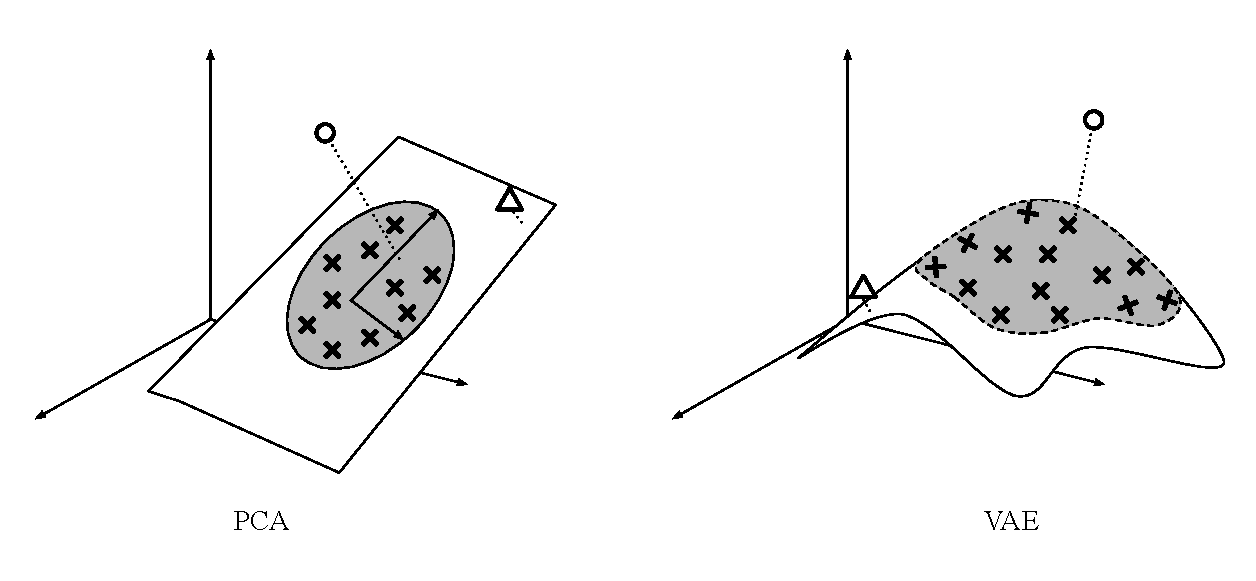
\includegraphics[width=0.9\textwidth]{PCAvsVAE.pdf}
			\caption{\textcolor{red}{\textbf{Figure 2 in the updated manuscript.} Illustration of the analogy between PCA and VAE. Closed regions describe the lower-dimensional manifold the in-control distribution lies in. The crosses represent the in-control samples observed in Phase-I and the gray region represents the subset of the lower-dimensional manifold where in-control samples are typically sampled from. The observation represented with a circle is typically detected with $ Q $-statistic and the observation represented with a triangle is typically detected with $ \Tsq $-statistic.} \label{fig:pcaVSvae}}	
		\end{centering}
	\end{figure}
}


\item On page 12, I recommend rewording the statement \textquotedbl Our
first major claim is that latent variable-based statistics are not
useful for profile monitoring ...\textquotedbl{} I think you mean
that using only (9) (the T\textasciicircum 2-like component) by itself
is not useful. But since (10) can also be viewed as a latent variable-based
statistic, the current wording sounds like you are saying that using
(9) and (10) together are not useful.

\textbf{\uline{Ans:}} Thank you for this important suggestion.
Given that the models we are using belong to the latent-variable models,
it is quite understandable that the word ``latent variable-based''
may cause confusions on which statistics it actually refer to, either
(9) or (10). 
\begin{itemize}
	\item To make it more clear, we will use the space in which
	these two monitoring statistics were computed to refer to these two
	statistics. Thus, we referred the statistics (10) as the ``residual
	space statistics'' and the statistics (9) as the ``latent space
	statistics''. Section 3.1 is where we first introduce these terms to the reader, right after we make the analogy between PCA and VAE monitoring statistics. The exact change is highlighted in red below. This way, the readers will internalize the analogy between them and the $ \Tsq $ and $ Q $ statistics, but without getting confused about all the notations that are being thrown around. From thereafter, we consistently use these terms in the rest of the paper.
\end{itemize}

{\color{red}{Observe that previously proposed formulations mentioned in \ref{sec:bckgrnd:critique} draw inspiration---directly or indirectly---from this framework. Statistics $R$ and $SPE$ are based on the $Q$-statistic. Let us call these \emph{residual space statistics}, as they rely on the sum of squared differences between the signal itself and its predicted value, \ie, residuals. The statistics $H^{2},T^{2}$ and $D$ are based on the $T^{2}$ of PCA. We call these \emph{latent space statistics}, as they rely exclusively on latent representations. }}


\item Why are you considering a VAE, as opposed to just an AE, i.e., why
do we need the variational part? By this, I mean why shouldn't we
omit any assumed distribution p(z) and just fit a regular autoencoder?
With a regular AE, we still have the encoded variables $z=\mu_{\phi}(x)$,
the decoded approximation $\mu_{\theta}(z)$, and the \textquotedbl residuals\textquotedbl{}
$x-\mu_{\theta}(z)$, so we could still consider the same two $T^{2}$-like
monitoring statistics for z and for the residuals. As I mention in
a comment below, I suspect part of the reason for the failure-to-extrapolate
is that the assumed p(z) acts like a regularizer and prevents some
of the z's from falling outside the normal region, even when the x
falls outside its region. Maybe you would not have this failure-to-extrapolate
problem if you use a regular AE instead of a VAE.

\textbf{\uline{Ans:}} Thank you for this comment. This is indeed
an interesting point. The major issue of using a regular AE is the
irregular latent space mapping and the challenge of setting the decision
boundary around this prior-free cloud of points related to the latent-space
statistics.

For example, one can think of a number of alternatives: (1) fitting
a multivariate Gaussian, (2) using a minimum enclosing hyperrectangle
(whether axis-parallel or arbitrarily oriented), (3) using average
distance to K-nearest neighbors or (4) fitting a Kernel density estimation
model. All these alternatives come with an implicit assumption around
the distribution of the in-control samples. More often than not, it
is very unlikely to guess which one will work best for any given dataset,
especially when deep learning based encoder-decoder structures are
used against very complicated datasets such as images.

To illustrate the ineffectiveness of the AE method, we ran another
set of experiments. For fairness, we kept the same convolutional encoder-decoder
architecture as in VAE for the real-case study. The experiments were
run on the same train-validation-test split of the rolling image datset.
We plot the encoded variables $z=\mu_{\phi}(x)$ below for when the
compressed length is 2, similar to the way we did it in the paper.
We also provide some decision boundary alternatives, in line with
our discussion above. We can observe that using regular AE does not
necessarily mitigate the issue in question. Other than classes 3,
5 and 6, none of the class encodings (shown in blue) really deviate
too much from the center of gravity of the validation points (shown
in red). Classes 3, 5 and 6 are not surprising either. They are the
ones that are picked up the most by latent space statistics (please
see column $H^{2}$ in Table 3 in page 28 of the old manuscript or Table 3 of the new manuscript). This suggests that AE
and VAE behave quite similar regardless of the regularization brought
up by VAE. Overall, we like to conclude that the lack of the extropolation
issue is an inherent problem of deep neural network including both
VAE and AE, which has been discussed in Appendix. B. As a result,
we kindly reject the suspicion that VAE regularization is the culprit.

Finally, we would like to mention that the advantage of the residual
space statistics for the VAE method compared to the AE method for
anomaly detection has been proved in many papers including {[}1{]},
which is not the major focus of this paper. In this paper, we emphasize
more on finding the most efficient and effective statistic for VAE
methods, which have been proved to be very useful for anomaly detection
in literature {[}1{]}.

\begin{figure}[H]
\captionsetup{labelformat=empty}
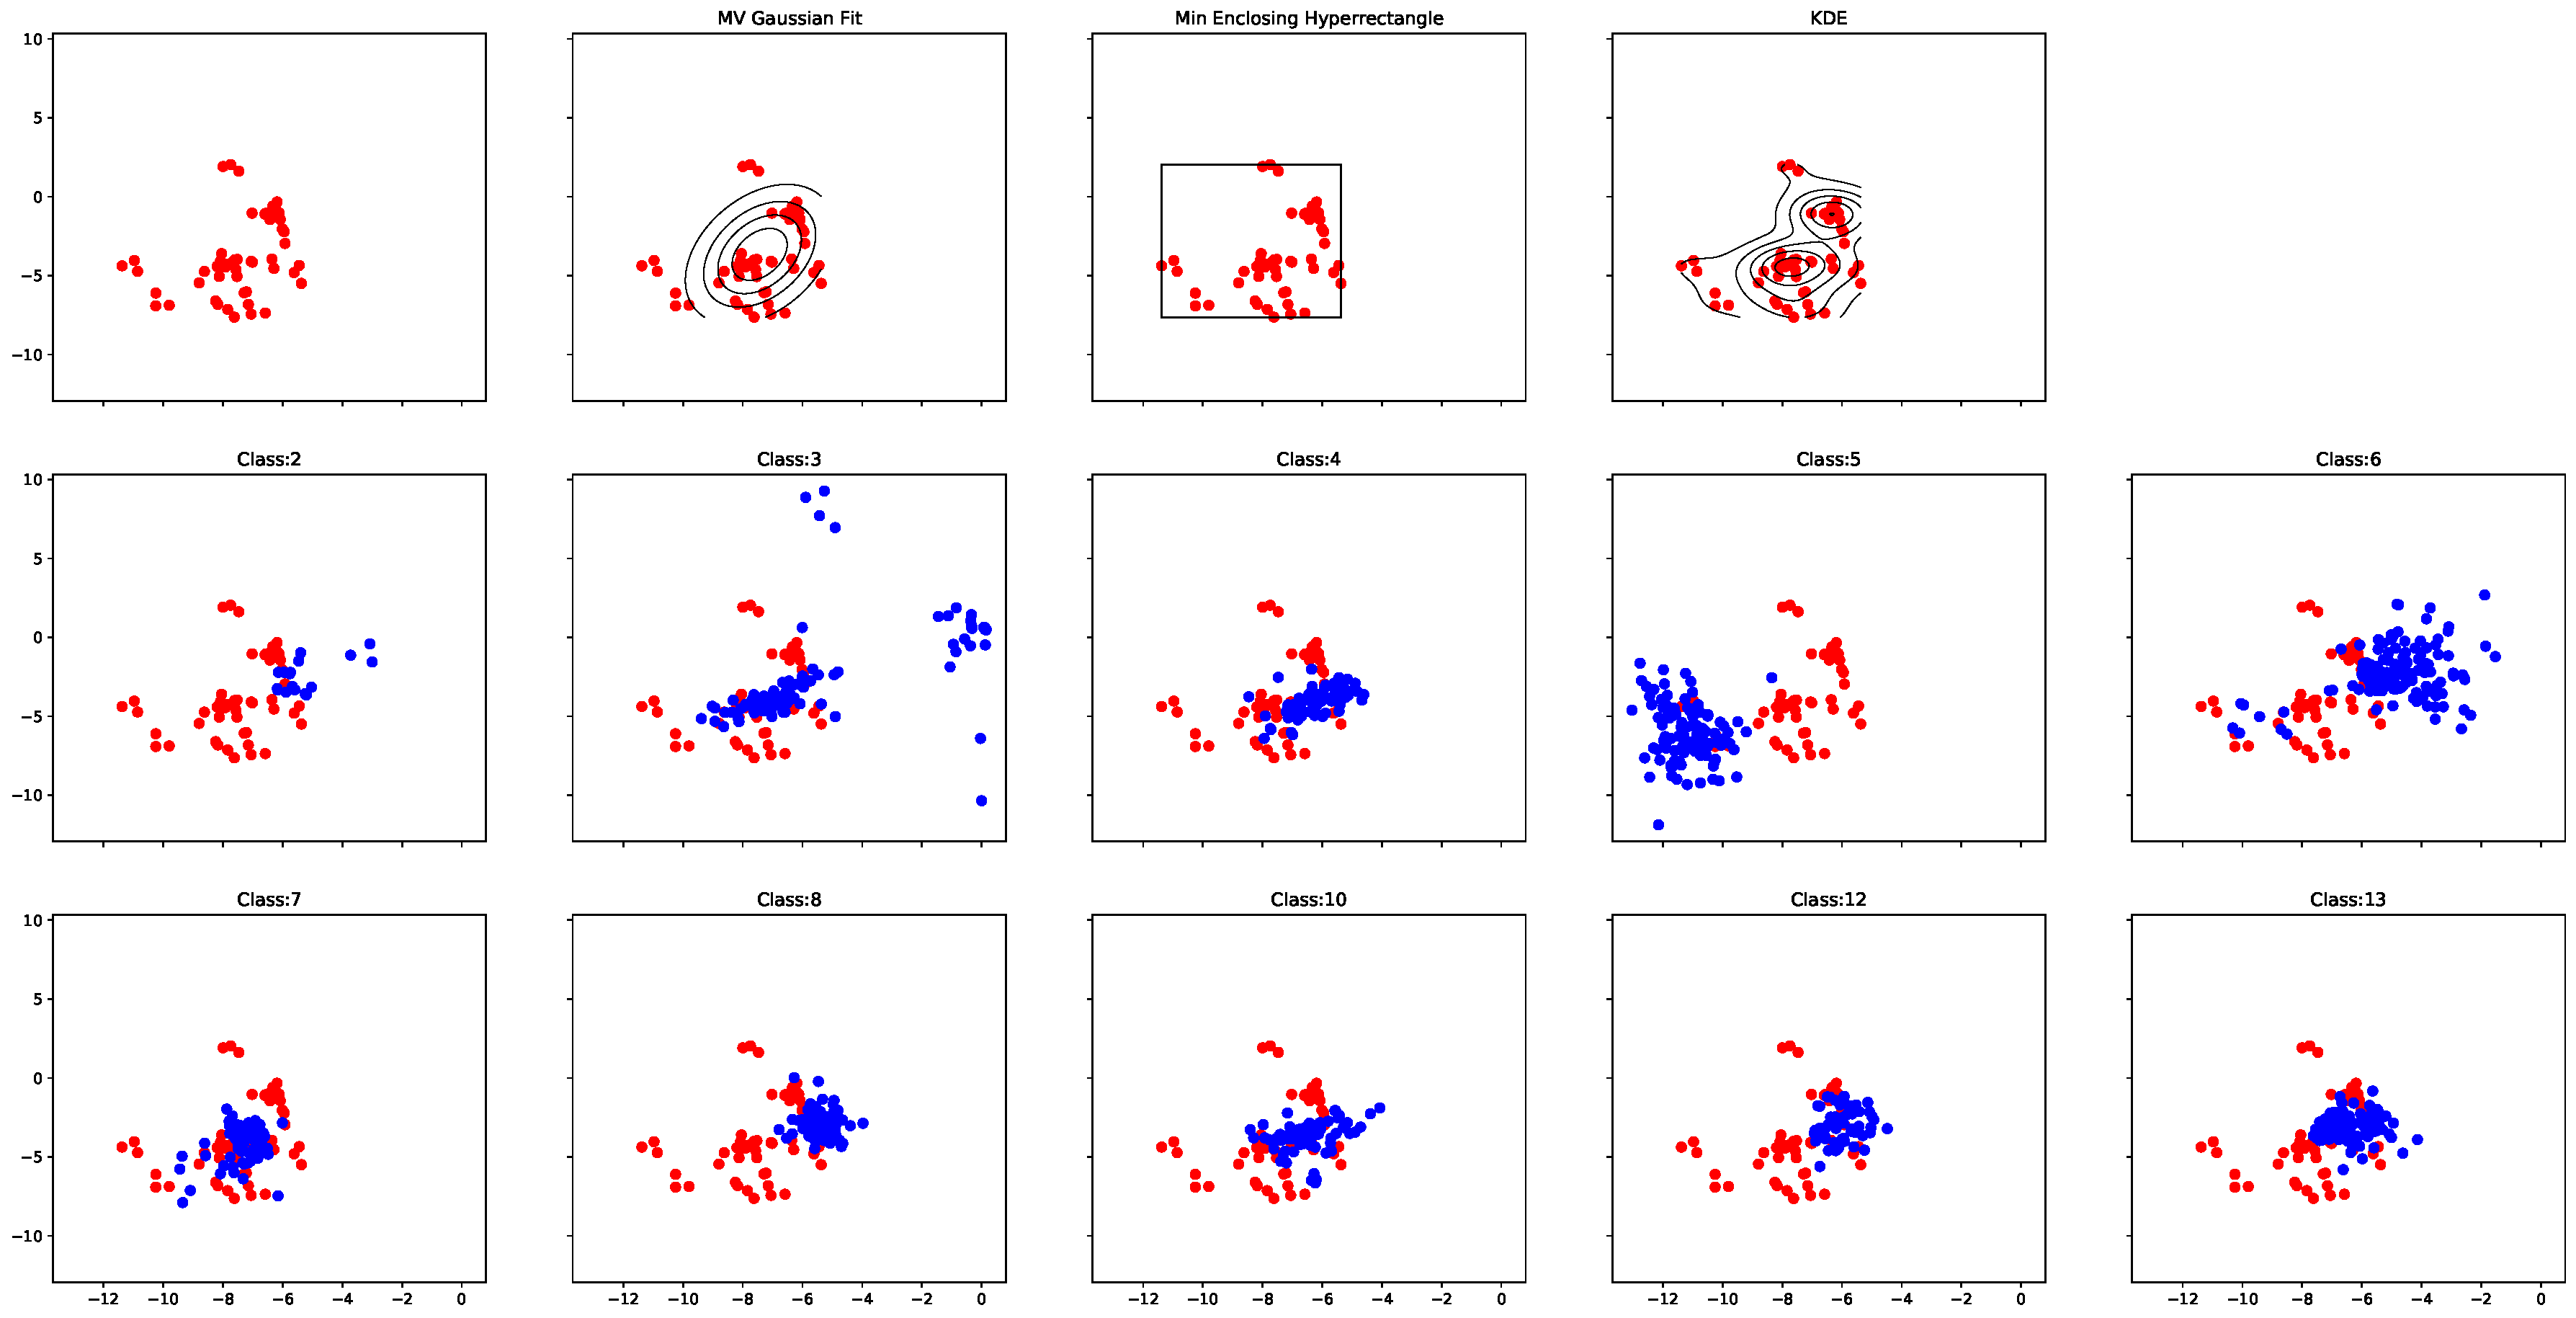
\includegraphics[scale=0.2]{scatter}

\caption{Encoded variables with a regular AE. Validation samples are shown
in red. Out-of-control class samples are shown in blue. Black lines
indicate the contours of the fit wherever applicable.}
\end{figure}

{[}1{]} An, Jinwon, and Sungzoon Cho. \textquotedbl Variational autoencoder
based anomaly detection using reconstruction probability.\textquotedbl{}
Special Lecture on IE 2.1 (2015): 1-18.
\item Regarding point 1 on page 12: For the standard linear PCA-based monitoring,
it is well known that only monitoring the dominant PC space misses
shifts that occur outside of this space. I recommend including an
older reference on this, and relating your point to the analogous
point for linear PCA. This will help JQT readers (who are familiar
with the linear situation) to better relate to the nonlinear situation.

\textbf{\uline{Ans:}} Thank you for this comment. We agree
that the previous ``Point 1'' is misleading for our readers. The enumeration has been discarded during the restructuring of the paper.

\begin{itemize}
	\item The argument you are referring to in your comment roughly refers to using $ Q $ alongside with $ \Tsq $ because $ \Tsq $ by itself is not enough for monitoring with PCA. The argument we make in this paper takes this argument further and suggests that if VAE used instead of PCA, only $ Q $ should be used. Therefore Point 1 was rather irrelevant to our argument, therefore we discarded it. Instead, especially in Section 3.2, we focused on why $ \Tsq $-like statistics (\ie, latent space statistics) are unreliable which we relate to the incorrect latent mappings produced by VAE.  The probabilistic equivalent of "monitoring dominant PC shifts" is what we explain in the paper as monitoring the shift in the prior distribution $ \pz $. Unlike how previous papers claim, latent space statistics cannot be trusted to detect such shifts. Instead, residual space statistics can do that too, in addition to being able detect shifts in the condition distribution $ p(\mbx \g \mbz) $. To reflect this change, we added a new, more concise enumeration of our argument in the introduction part of Section 3.2:
\end{itemize}

{\color{red}
There are two major pitfalls of the previously proposed methodologies:
\begin{enumerate}
	\item Latent space statistics $H^{2},T^{2}$ and $D$ or any other formulation that relies exclusively on the latent representation $ \mbz \sim \qphizgivenx{\mbz}{\mbx}$ will be unreliable for process monitoring. Thus, they should be discarded altogether from the monitoring framework since they will likely increase false alarms without contributing to the detection power in any meaningful way.
	\item Residual space statistic $ SPE $ and $ R $ rely on Monte Carlo sampling. These are not computationally feasible given how expensive calculations are on deep neural networks. An alternative approach is required to stay computationally feasible without sacrificing too much from the estimation quality of these statistics.
\end{enumerate}
}

\item Figure 2 and Point 2 on page 13 needs a lot more elaboration. It is
making an important argument, but I don't think readers without strong
machine learning background will follow with the current level of
detail.

\textbf{\uline{Ans:}} Thank you for this suggestion. We certainly
agree with it. 
\begin{itemize}
	\item We substituted Figure 2, which is now Figure 3 in the paper. We also include that figure below for your convenience.
	\item In line with your comments about the paper
	being accessible by JQT audience, we also skimmed the details about
	the properties of latent representations, such as disentanglement
	or invariance to nuisance factors. 
	\item The main idea that we want to convey
	to the readers in that section is the unreliability of the semantics
	of deep encoder learned latent representations when it comes to profile
	monitoring. This is why, with the help of the new figure, we updated Section 3.2.1, which is highlighted below.
\end{itemize}

{\color{red}
	First, we focus on the unreliability of latent space statistics. Let us first start with the case when the shift occurs in the latent distribution (i.e., $\pz$). According to the PCA-VAE analogy illustrated in Figure 2, latent space statistics are supposed to catch such shifts, which are represented with triangular points in the same figure. While this may work for PCA-based monitoring, we claim that such an analogy cannot be straightforwardly made for VAE because neural network-based encoders in autoencoder architectures typically learn incorrect mappings of actual latent variations. We illustrate this phenomenon in Figure 3. The line segment ABC illustrates a traversal along a latent dimension. All the samples generated along the line segment AB are sampled from the typical region of the in-control process and their mappings are contained within the typical region of the predicted space. However, Point C is generated by an out-of-control process where there is a shift in latent distribution but its mapping incorrectly falls within the probable region. This leads to false evidence which suggests that Point C is unlikely to be generated by an out-of-control process while in reality, it was.
	
	The reasons as to why incorrect mappings are learned by deep autoencoders have been studied well in the deep learning literature. Interested readers are encouraged to refer to \textcite{AchilleS18} for a discussion of the properties of ideal latent representations and to \textcite{locatello2018challenging} for a discussion of the challenges around attaining one of these properties, namely, disentanglement. The key takeaway is that it is very likely that we end up with an imperfect mapping, especially with real-life datasets. Consequently, in Phase-II, samples generated by out-of-control processes that are characterized by a shift in the latent distribution will not be mapped consistently to the regions in the latent space which we consider to be unusual. This will result in an increased type-II error.
	
	A natural question to ask at this point is how should we expect to detect shifts in latent distribution if we cannot rely on latent representations. We argue that an analogue of a $ Q $-chart would catch such shifts too, even though its original purpose is to catch shifts in the conditional distribution. Our argument is based on another shortcoming of neural networks, namely, failure to extrapolate. Deep neural networks approximate well only at a bounded domain defined by where the training set is densely samples from. In the context of our problem, this refers to the high-density region of $ p(\mbx) $ which generated the set of in-control profiles we use in Phase-I. The behavior of the function is unpredictable and often erroneous outside the training domain. In other words, it does not extrapolate well beyond the domain of training samples, which are likely to be coming from out-of-control processes. We refer interested readers to Appendix B, where we replicate this phenomenon on a toy example.
	
	A decoder that fails to extrapolate is counter-intuitively helpful since it will struggle with generating profiles that are in the low-density region of the in-control data distribution $ p(\mbx) $. This means that the discrepancy between the true profile and its generated counterpart will be larger for out-of-control profiles than it is for in-control profiles, regardless of the source of the shift. Thus, a monitoring statistic that is based on the residuals only would be efficient at covering both sources of shifts. We refer the reader back to Figure 3 for an illustration. There is a significant discrepancy between the observations and reconstructions of Point C and D, even though they are generated by different sources of shifts in the process. Thus, an extension of a residual space statistic should be able to catch both types of shifts.
}

\begin{figure}[h]
	\captionsetup{labelformat=empty}
	\begin{centering}
		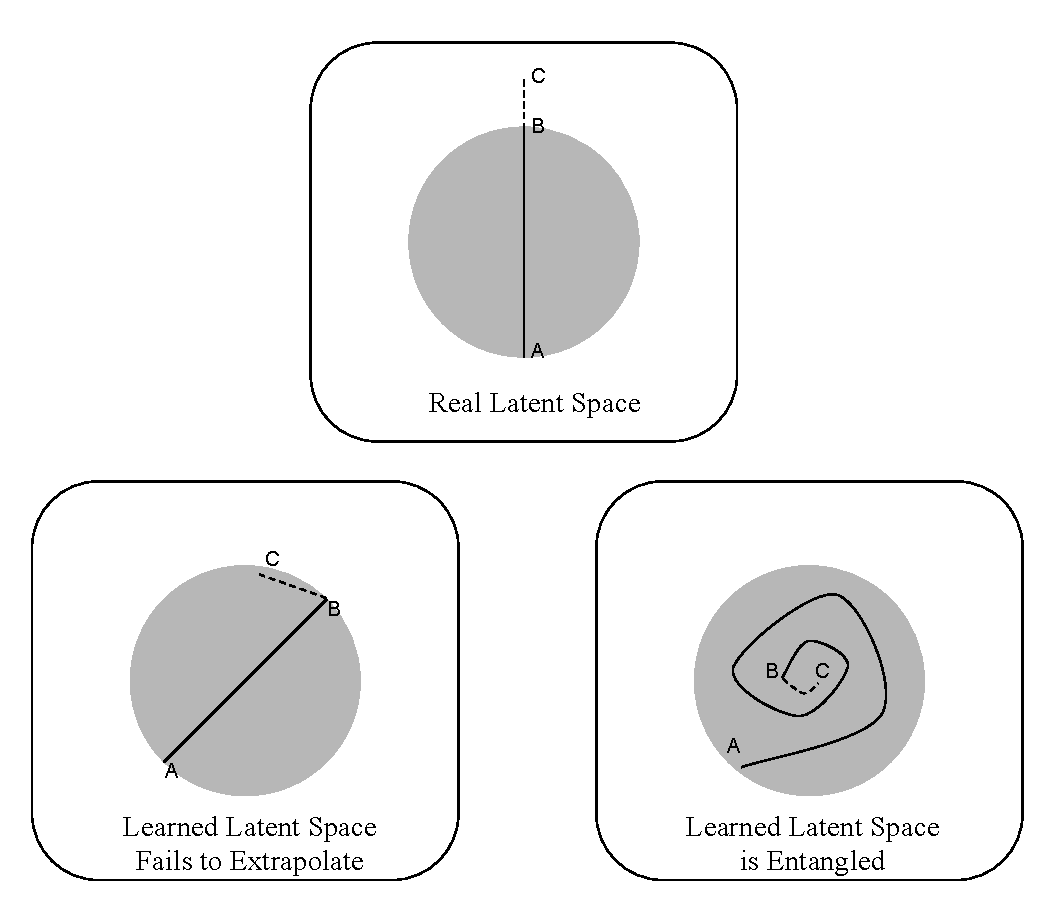
\includegraphics[width=0.9\textwidth]{Disentangled_Extrapolated.pdf}
		\par\end{centering}
	\caption{\color{red}\textbf{Figure 3 in updated manuscript.} Illustration of incorrect latent mappings phenomena and how process control fails in latent space. \textbf{Bottom left:} The true latent variations of in-control samples are generated from the gray region, which is the probable region. Point A and Point B are extreme values along a dimension of variation. Point C is generated by an out-of-control process with a shift in latent distribution. Point D is generated by an out-of-control process with a shift in the residual distribution. The predicted counterpart of each point is denoted by an apostrophe (\eg, A' for A). \textbf{Top Left:} Observations of true latent variation in the high-dimensional space that lie close to a low-dimensional manifold. \textbf{Top Middle:} The encoder and decoder of VAE trained exclusively with in-control samples (\ie, the gray region in the observed space). \textbf{Bottom Middle:} Incorrectly mapped variation in the predicted latent space where the gray region is the probable region. \textbf{Top Right:} Reconstructions of the variation in high-dimensions, with a failure in extrapolation beyond the in-control region. \label{fig:entang-extrap}}
\end{figure}

\item Further regarding Point 2: The crux of the failure-to-extrapolate
issue is that unusual x values might get mapped to typical z values,
and therefore cause false negatives. Is this because of the structure
of the decoder part (which might suggest a different structure could
be more suitable for this type of VAE-based process monitoring), or
is it because of the implicit regularization of z when fitting the
VAE via the assumed p(z), or both. I suspect the latter is just as
important if not more important, but Appendix B focuses on the former.
Could this problem be solved by using a regular AE instead of a VAE
(per my earlier comment)? Or could it be solved by replacing the Gaussian
p(z) that is used during the fitting stage with a heavier tailed distribution
(e.g. multivariate t, or mixture of Gaussian and uniform over a much
larger support) during the monitoring stage? If the same Gaussian
p(z) is used during monitoring as during fitting the VAE, this is
like telling the control chart that you expect the data during monitoring
to behave the same as the data during fitting, i.e., that process
shifts are not likely to happen. The Gaussian/uniform mixture p(z)
would allow you to specify \textquotedbl prior\textquotedbl{} probabilities
on how likely a shift is to occur.

\textbf{\uline{Ans:}} Thank you for this comment. Unfortunately, we are not sure if we understood your comments well. We will answer based on two alternatives of what we think you meant in your comments.
\begin{itemize}
	\item Alternative 1: You are suggesting using Gaussian $ \pz $ to fit VAE with in-control profiles. But you are suggesting that a different distribution should be used for Phase-II. We don't understand how one could use a different distribution for the monitoring stage. The purpose of Phase-II monitoring is to check if an incoming profile adheres to the in-control behavior, which by definition only calls for a single distribution, which is the distribution of the in-control process. If you replace the distribution in Phase-II, which dataset are you going to fit its parameters with? Because in practice, you will not have access to profiles from out-of-control process. Besides, the deep learning architecture limits you to the initial distribution you fitted it with. The typical VAE can only produce a mean and a diagonal covariance for a Gaussian distribution whether in training or inference stages. Even if changing distributions made sense, you'd still have to train another model with a different architecture.
	\item Alternative 2: You are suggesting replacing Gaussian prior altogether, and using a different distribution both at training and test stages. This may not be as straightforward if the KL-divergence (or any other distance measure) between the proposed prior and what the encoder infers has a closed-form, differentiable formulation. For the sake of discussion, let us assume that this is not a problem. Even in that case, if you used a heavier-tailed distribution, the inferred means of in-control and out-of-control samples will simply disperse out together and relative decisions would be unchanged. The control limit will simply be relaxed a a bit more. We find the mixture suggestion to be the most promising and interesting. However, to train such a model, one would again need at least some amount of out-of-control data at training time. Even if we had that (maybe by keeping the outliers found in Phase-I), the priors would not reflect the likelihood of a shift to occur at Phase-II but the frequency of outlier data within the training set. If those probabilities didn't match, we would have a problem.
	\item Our response to your suggestion about using regular AEs are answered in the response to your comment 5.
\end{itemize}

\item Section 4.1: I don't recognize this as the gasket bead example from
Shi, Apley and Runger (2016). It might represent some other type of
bead that changes position/shape, but it doesn't seem to have much
connection to gaskets.

\textbf{\uline{Ans:}} Thank you for this comment. It is our mistake that we kept the wording gasket bead because just as your comment suggests, a 2D point cloud with a circular shape does
not have much connection to the gasket bead component anymore, even though the semantics of location and shape variations have similarities. As a response:
\begin{itemize}
	\item We made sure all the related wordings are changed to dome, which is a better descriptor of the topology of our simulation generating process.
\end{itemize}  

\item Additional comments that are minor by themselves but related to the
bigger problem of poor writing in general:
\begin{itemize}
\item First paragraph of intro: In \textquotedbl ... intra-sample variation
lies on a nonlinear low-dimensional manifold\textquotedbl{} it is
not clear what \textquotedbl sample\textquotedbl{} means. Does \textquotedbl intra-sample
variation\textquotedbl{} just mean variation across a sample of parts,
items, images, etc? Please clarify.

\textbf{\uline{Ans:}} Thank you for this comment. You are right
to call out ``sample'' as an ambiguous word. In that sentence, we
mean profile-to-profile variation. Therefore, we made the following
change:
\end{itemize}
\textcolor{red}{Specifically, we focus on the case where profiles
are observed in a high-dimensional space but profile-to-profile variation
lie on a nonlinear low-dimensional manifold.}
\begin{itemize}
\item Page 5, 3rd contribution bullet: It sounds like you are saying latent
variable-based monitoring should not be used, but it seems the entire
paper is about latent variable-based monitoring. VAEs are latent variable
models. Please clarify.

\textbf{\uline{Ans:}} Thank you for this comment. Please see the
our answer to you comment 4. In there, we explain how we rename this
to ``latent space statistic''. We agree with your comment on this.
\item In Eq. (5), I can't find where \textbackslash mu\_\{\textbackslash phi\}(x)
has been defined. I can guess what it is, but readers shouldn't have
to guess. There are quite a few other undefined or unclearly defined
notations.

\textbf{\uline{Ans:}} Thank you for this comment. We added the
following sentence to Section 2.1:
\end{itemize}
\textcolor{red}{The encoder is modeled as another Gaussian distribution
$\encoding=\Norm(\mbz;\mu_{\mbphi}(\mbx),\sigma_{\mbphi}(\mbx))$
where the mean and standard deviation of the proposal distribution
are inferred via high capacity neural networks $\mu_{\mbphi}$ and
$\sigma_{\mbphi}$, respectively.}
\begin{itemize}
\item On page 11, does \textquotedbl this is actually true for linear latent
variable models\textquotedbl{} mean \textquotedbl this holds exactly
for linear latent variable models\textquotedbl ?

\textbf{\uline{Ans:}} Thank you for this comment. This sentence
has been discarded during revision regarding other comments.
\end{itemize}
\end{enumerate}
\printbibliography

\end{document}
